Le seguenti analisi hanno lo scopo di rilevare come la presenza di possibili relazioni tra alcune caratteristiche (o parametri) del sistema possano influire sul comportamento di emergente della simulazione.
Per effettuare tali analisi, poiché si tratta di un sistema complesso, è stato necessario effettuare un insieme di simulazioni in modo tale da raccogliere i dati che derivano dal comportamento emergente.
Poiché in questa Sezione si presentano analisi differenti tra loro, ogni volta verrà descritta la metodologia utilizzata per la raccolta dei dati.
Si tenga presente che il metodo di prioritizzazione delle celle dovuto alla segnalazione di feriti segue la strategia che attribuisce una priorità fissa alle celle del vicinato.
Gli studi effettuati sono i seguenti:\begin{itemize}
	\item come il numero dei robot influisce sul numero di ripetitori rilasciati e come fa variare il valore di \textit{fitness};
	\item come la dimensione della mappa influisce sul numero di ripetitori che devono venir rilasciati dagli agenti;
	\item come la difficoltà totale della mappa influenza il numero di \textit{step} richiesto per completare l'esplorazione.
\end{itemize}
\subsection{Studio sul numero di robot}
\label{subsec:nrobots}
Come già detto, sul variare del numero dei robot sono state effettuate due analisi riguardo due aspetti diversi del sistema.
In entrambi i casi, però, la metodologia di raccolta dati è stata analoga: per tutte le simulazioni effettuate si è mantenuta la stessa mappa di dimensioni 30$\times$30, mappa che abbiamo verificato non presentasse al suo interno casi patologici (\textit{e.g.}, grandi zone inesplorabili poiché irraggiungibili o non visibili).
Inoltre, per i valori di $\alpha$, $\gamma$ e per il raggio dei sensori sono stati utilizzati i dati inferiti dal processo di ottimizzazione descritto nel Capitolo \ref{chap:pso}. Il \textit{range} del ripetitore è stato mantenuto pari a 3 celle, in modo da avere risultati scalati correttamente rispetto alle dimensioni che erano state considerate originariamente (mappe 333$\times$333 con ripetitori con una portata di 30 celle). Infine, per ogni valore del numero di robot, sono state effettuate 10 simulazioni e i feriti potevano segnalare la loro presenza.

Per quanto concerne \margin{Numero di robot \textit{vs} ripetitori rilasciati}il numero di ripetitori rilasciati, come mostrato in Figura \ref{fig:robotsbeans}, tale numero aumenta all'aumentare dei robot impiegati nonostante le dimensioni della mappa rimangono costanti.
Tale comportamento può essere considerato ragionevole perché, all'aumentare del numero dei robot, aumentano i casi in cui due agenti escono contemporaneamente dalla zona coperta e quindi rilasciano due ripetitori la cui area coperta di uno dei due sarebbe bastata per coprire anche parzialmente l'area dell'altro.
Di fatto, i robot non hanno alcun meccanismo di coordinamento per la creazione della rete, ognuna pensa a sé e quindi all'aumentare del numero di robot aumentano i casi in cui due robot rilasciano due ripetitori vicini tra loro, non ottimizzando l'utilizzo del singolo ripetitore e portando quindi a molte porzioni di territorio coperte da più di un singolo ripetitore.
Si fa presente che tale numero non è distorto dal fatto che ogni singolo robot rilascia un ripetitore appena viene disposto sul campo, poiché i robot rilasciano il ripetitore solo se in quella cella non è già presente un ripetitore.
\begin{figure}
	\centering
	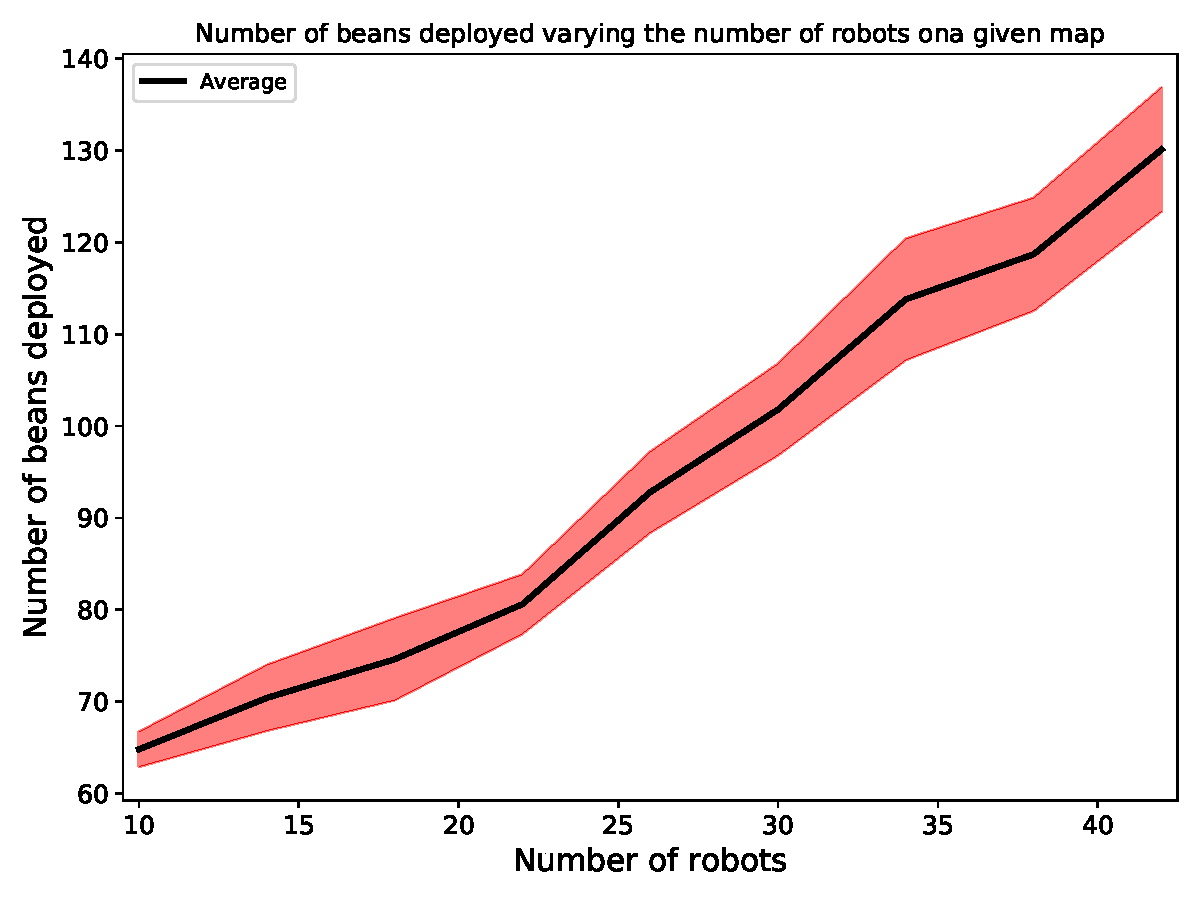
\includegraphics[width=0.9\linewidth]{images/macro_results/robots_beans}
	\caption{In Figura è rappresentato come il numero di robot influisce sul numero di ripetitori rilasciati nel territorio. Sull'asse delle \textit{x} è presente il numero di robot e sull'asse delle \textit{y} il numero di ripetitori disposti. Sono state effettuate 10 simulazioni per ogni valore di numero di robot, in nero è presente la media del numero di ripetitori rilasciati e l'area rossa indica la deviazione standard.}
	\label{fig:robotsbeans}
\end{figure}

Rispetto alla seconda analisi effettuata, si ricorda che il valore di \textit{fitness} è quello definito nella Formula \ref{math:pso}.
Per quanto riguarda i risultati ottenuti e mostrati in Figura \ref{fig:fitness}, si nota come con fintanto che il numero di robot resta basso, la \textit{fitness} diminuisce velocemente, in quanto il tempo di esplorazione del territorio diminuisce significativamente. Al contrario, con un numero elevato di agenti, il valore di \textit{fitness} diminuisce molto più lentamente, perché il tempo di esplorazione non subisce diminuzioni significative e nel mentre vi è un numero sempre maggiore di robot in stato di \textit{idling} mentre ci si approccia al termine dell'esplorazione.
Si fa presente che i valori rappresentati dai punti in rosso sono il valore medio di \textit{fitness} che si è ottenuto con tale numero di robot, mentre le barre nere (poco visibili) indicano la variazione data dalla deviazione standard; il fatto che spesso non si vedano è dato dal fatto che la deviazione standard è molto bassa.
Considerando il grafico mostrato e concentrandosi sull'intervallo tra i 51 e 76 robot, ci si pone una domanda aperta a cui servirebbero analisi di costi successive e non rientranti nei termini di questo lavoro: “vale la pena utilizzare 10, 15 o addirittura 25 robot in più se il valore di \textit{fitness} e il tempo di esplorazione diminuiscono così poco?”.\\
Pensiamo che per rispondere a questa domanda (escludendo i dibattiti etici a riguardo) sia necessario fare delle analisi che tengano conto del costo di realizzazione dei robot, di quanti robot si hanno a disposizione in scenari realistici e se sia necessario intervenire su un solo quartiere o più quartieri.
\begin{figure}
	\centering
	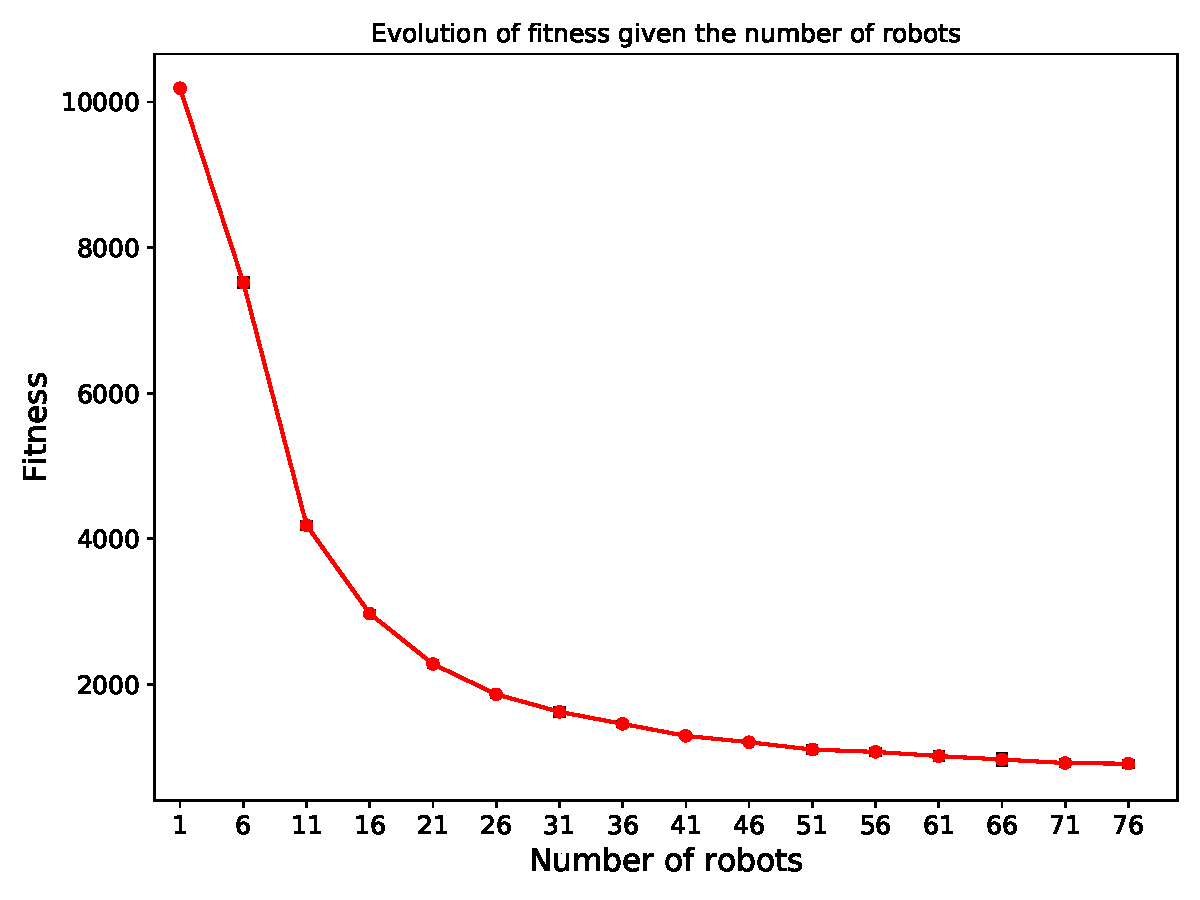
\includegraphics[width=0.9\linewidth]{images/macro_results/fitness}
	\caption{Sull'asse delle \textit{x} è indicato il numero di robot, su quello delle \textit{y} il valore di \textit{fitness}. Poiché per ogni valore sono state effettuate 10 simulazioni, i punti rappresentati sono la media mentre in nero sono rappresentate le barre di errore date dalla deviazione standard, poco visibili poiché i valori di deviazione standard sono molto piccoli rispetto alle scale del grafico.}
	\label{fig:fitness}
\end{figure}

\subsection{Dimensioni della mappa \textit{vs} numero di ripetitori rilasciati}
Per la produzione di questa analisi, sono state effettuate 10 simulazioni per ogni dimensione della mappa considerate, le mappe sono state generate casualmente ad ogni simulazione, per i parametri sono stati utilizzati i valori inferiti dal processo di ottimizzazione (si veda il Capitolo \ref{chap:pso}), il raggio dei ripetitori pari a 3 celle, i feriti erano in grado di poter segnalare la loro presenza e il numero di robot e il numero di robot era pari a $1/5$ di \texttt{ncell} (arrotondato per eccesso).
I risultati mostrati in Figura \ref{fig:beans}, dove la linea nera è la media e l'area in rosso rappresenta la deviazione standard, mostrano che all'aumentare della dimensione del territorio il numero di ripetitori rilasciati aumenta (come supposto) in maniera assimilabile qualitativamente ad una crescita quadratica.
Questo risultato è più che ragionevole considerando come l'aumentare della dimensione del lato dalla mappa fa aumentare l'area di un quadrato, portando quindi ad una crescita quadratica delle dimensioni che si riflette coerentemente nel numero di ripetitori necessari.
È interessante notare, aggregando questo dato a quello presentato nella Sotto-sezione \ref{subsec:nrobots}, che l'aumento del numero di ripetitori disposti viene influenzato maggiormente dal numero di agenti impiegati e dal fatto che non si coordinano tra loro, rispetto alle dimensioni effettive della mappa che comporta una crescita che è intrinseca con l'aumento delle dimensioni della mappa.
\begin{figure}
	\centering
	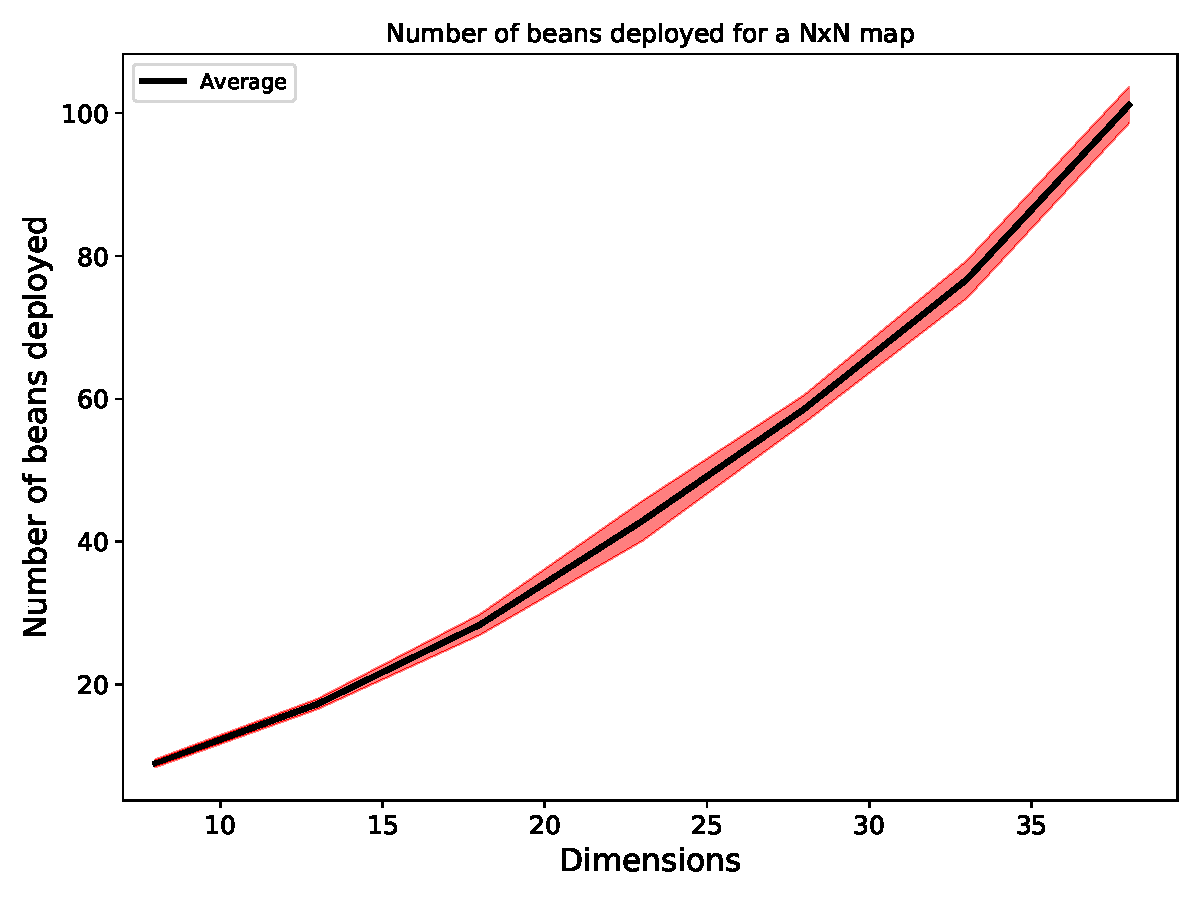
\includegraphics[width=0.9\linewidth]{images/macro_results/beans}
	\caption{Figura che rappresenta come all'aumentare delle dimensioni del territorio (sull'asse delle \textit{x} è rappresentata la dimensione del lato della mappa) aumenta il numero di ripetitori (sull'asse delle \textit{y}) necessari per coprire tutta l'area. In nero è rappresentato il valore medio, mentre in rosso la deviazione standard.}
	\label{fig:beans}
\end{figure}

\subsection{Difficoltà della mappa \textit{vs} tempo richiesto}
Per tale studio, sono state effettuate un totale di 7 simulazioni in cui è stata fatta aumentare la dimensione della mappa, e con esso in maniera proporzionale il numero di robot impiegati, in modo tale da far aumentare la difficoltà complessiva; per difficoltà complessiva si intende la somma della difficoltà di ogni singola cella.
Le mappe sono state generate casualmente e si è deciso di non effettuare più simulazioni per ogni difficoltà per non complicare inutilmente il grafico e il processo di generazione dati in aggiunta a tutto il tempo richiesto da tali simulazioni. Inoltre, i risultati ottenuti da queste poche simulazioni sono stati considerati soddisfacenti per delle analisi di massima.
Siamo anche convinti che effettuare analisi di fino su queste quantità richiederebbe di prendere in considerazione un numero elevato di fattori, e i risultati prodotti potrebbero non risultare interessanti o significativi, soprattutto considerando che nella pratica ogni situazione sarà unica e poco prevedibile a priori. Lo scopo di questa analisi è semplicemente individuare l'andamento medio del tempo richiesto al crescere della difficoltà totale.\\
Per quanto riguarda i risultati riportati in Figura \ref{fig:difficulty}, si nota che anche in questo caso l'aumento di \textit{step} richiesti per completare l'esplorazione non è lineare rispetto alla difficoltà ma presenta piuttosto un andamento più assimilabile a quello di un logaritmo.
In aggiunta a tale prima analisi non è possibile trarre ulteriori conclusioni significative, servirebbero molte più simulazioni e sarebbe necessario definire una strategia non triviale per poter tenere in considerazioni più fattori per proporre un'analisi approfondita di tale relazione.
\begin{figure}
	\centering
	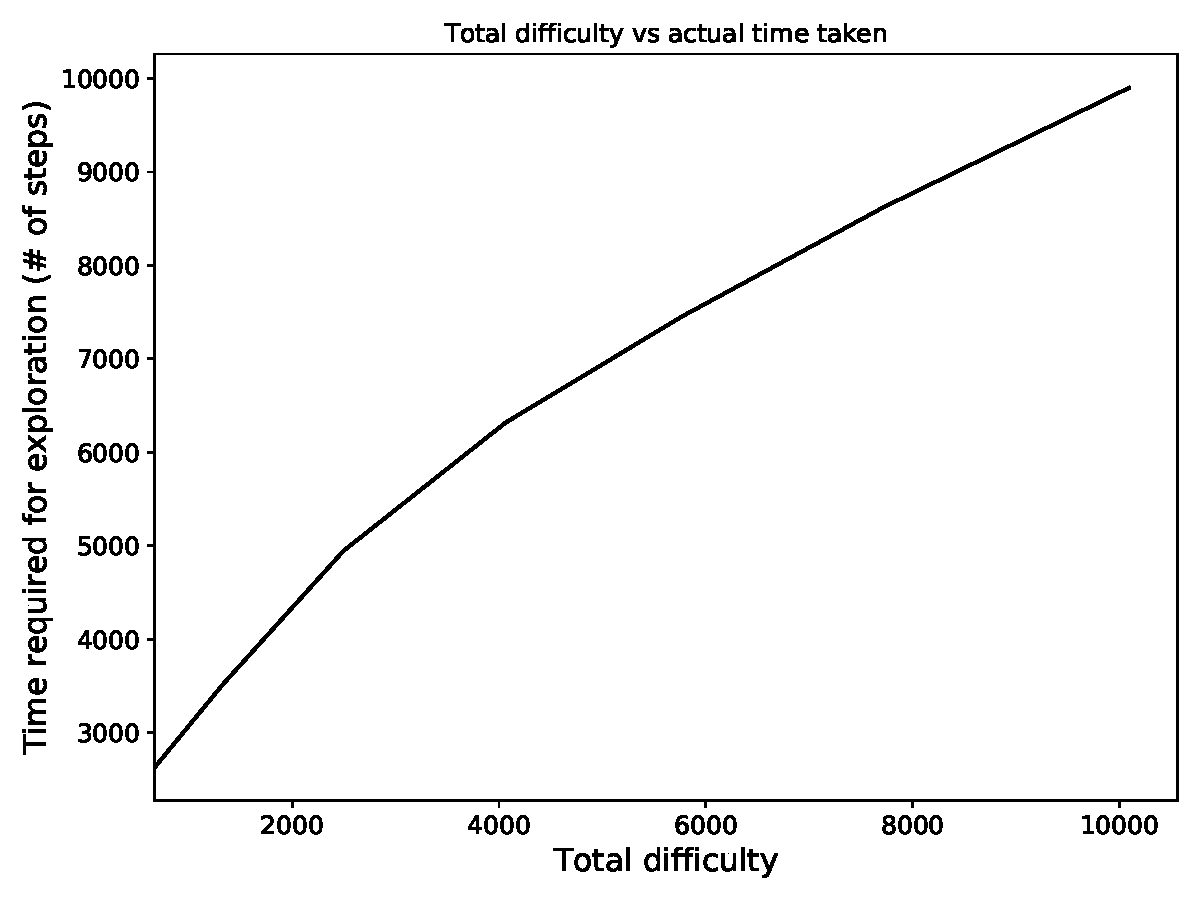
\includegraphics[width=0.9\linewidth]{images/macro_results/difficulty}
	\caption{Sull'asse delle \textit{x} è presente la difficoltà complessiva di esplorazione della mappa e sull'asse delle \textit{y} il numero di \textit{step} effettuati per completare l'esplorazione.}
	\label{fig:difficulty}
\end{figure}
\newpage